\begin{frame}{Introducción}
\justifying
La Programación Orientada a Objetos (POO) es un paradigma fundamental en la programación para el desarrollo de cualquier software. A la fecha son la mayoría de lenguajes de alto nivel los que llegan a soportar la POO. como son Java, C\#, C++, Python, etc.

Por esta razón hablaremos de esta forma de pensar, de este paradigma que es la POO.

{\tiny Python Manizales - Jesse Padilla Agudelo}
\end{frame}

\begin{frame}{Introducción}
\justifying

\begin{figure}[H]
\centering
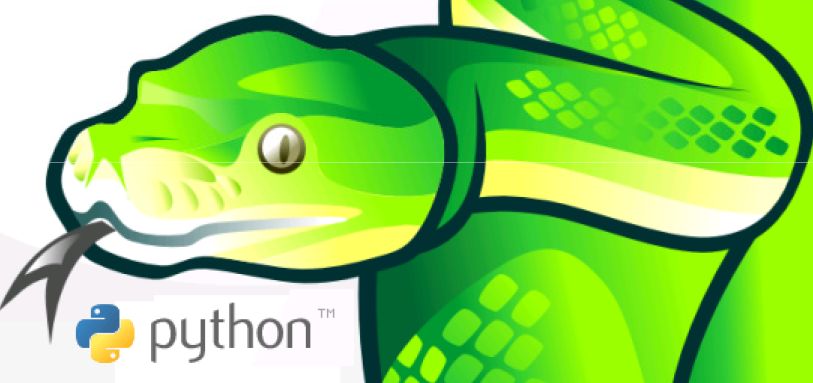
\includegraphics[scale=0.25]{Section_Files/images/01.png}
\caption{Imagen popular que asocia al lenguaje Python.}
\end{figure}

{\tiny Python Manizales - Jesse Padilla Agudelo}
\end{frame}

\begin{frame}{Programación Orientada a Objetos}
\justifying
La programación orientada a objetos es un paradigma de programación que busca representar entidades u objetos agrupando datos y métodos que puedan describir sus características y comportamientos.

{\tiny Python Manizales - Jesse Padilla Agudelo}
\end{frame}

\begin{frame}{Programación Orientada a Objetos}
\justifying
La POO paradigma de programación en el que los conceptos del mundo real relevantes para nuestro problema se modelan a través de clases y objetos, y en el que nuestro programa consiste en una serie de iteracciones entre estos objetos.

{\tiny Python Manizales - Jesse Padilla Agudelo}
\end{frame}

\begin{frame}{Ventajas de la POO}
\justifying
\begin{itemize}
\item Fomenta la reutilización y extensión del código.
\item Permite crear sistemas más complejos.
\item Relacionar el sistema al mundo real.
\item Facilita la creación de programas visuales.
\item Construcción de prototipos.
\item Agiliza el desarrollo de software.
\item Facilita el trabajo en equipo.
\item Facilita el mantenimiento de software.
\end{itemize}

{\tiny Python Manizales - Jesse Padilla Agudelo}
\end{frame}

\begin{frame}{Modelo Orientado a Objetos}
\justifying
\begin{itemize}
\item Objeto.
\item Clase.
\item Mensaje.
\item Método.
\item Interfaz
\item Herencia.
\end{itemize}

{\tiny Python Manizales - Jesse Padilla Agudelo}
\end{frame}